% =============================================================================
% Discriminative Parameter Splitting for LLMs (DPS-LLM) -- ACL Rolling Review
% =============================================================================
% Build:  pdflatex paper_acl && bibtex paper_acl && pdflatex paper_acl && pdflatex paper_acl
%
% ARR submission checklist (https://aclrollingreview.org/cfp):
%   * [review] option below => anonymous author block + line numbers (required
%     for submission). Switch to [final] for the camera-ready / preprint.
%   * Mandatory unnumbered "Limitations" section after the conclusion.
%   * Optional "Ethics Statement"; appendices after the references.
%   * Long paper: <= 8 pages of content (Limitations, references and
%     appendices do not count toward the limit).
% =============================================================================
\documentclass[11pt]{article}

\usepackage[review]{acl}   % <-- change to [final] for camera-ready

\usepackage{times}
\usepackage{latexsym}
\usepackage{amsmath}
\usepackage{amssymb}
\usepackage{booktabs}
\usepackage{graphicx}
\usepackage{microtype}
\usepackage{inconsolata}
\usepackage{array}
\usepackage{amsthm}
\newtheorem{theorem}{Theorem}
\newtheorem{proposition}{Proposition}

\title{Discriminative Parameter Splitting for Large Language Models: \\ Zero-Drift Network Expansion and Calculated Noise Symmetry Breaking}

\author{Muhammad Irfan \\
  SEECS, National University of Sciences and Technology \\
  Islamabad, Pakistan \\
  \texttt{mirfan899@gmail.com} \And
  Ali Tahir \\
  SEECS, National University of Sciences and Technology \\
  Islamabad, Pakistan}

\begin{document}
\maketitle

\begin{abstract}
Pre-training Large Language Models (LLMs) from scratch is compute-intensive, and a deployed model whose capacity saturates on a downstream task cannot easily be enlarged without discarding its checkpoint.
We present \textbf{Discriminative Parameter Splitting for LLMs (DPS-LLM)}, a progressive-growth method that doubles the intermediate width of every SwiGLU feed-forward block of a pre-trained Transformer while leaving its function unchanged at the moment of expansion.
DPS-LLM combines (i) a \emph{function-preserving} split---row duplication of the gate and up projections and column duplication of the down projection scaled by $\tfrac{1}{2}$---for which we prove exact output invariance, and (ii) \emph{Calculated Anti-Symmetric Noise}, a polarity-aware perturbation adapted from discriminative splitting of LSTM acoustic models, which breaks the gradient symmetry of duplicated neurons while cancelling first-order output drift.
We evaluate on two open-weight model families, \textbf{Qwen2.5-0.5B} (494M$\to$808M parameters) and \textbf{SmolLM-360M} (362M$\to$598M), fine-tuned on GSM8K and Alpaca-Cleaned with three seeds per condition, and compare DPS-LLM with the unexpanded model, exact duplication and isotropic Gaussian noise.
The split is function-preserving in practice: validation perplexity immediately after splitting is within $0.012$ of the base model, whereas omitting the $\tfrac{1}{2}$ factor raises it from $5.27$ to $14.85$.
The symmetry breaking, however, does not survive bfloat16: at the default noise scale the perturbation is almost entirely absorbed by rounding, the two copies of every neuron keep a cosine similarity of $1.0000$ throughout fine-tuning, and DPS-LLM, Gaussian noise and exact duplication are statistically indistinguishable (paired $t$-test, $p\geq0.09$).
Splitting doubles the relative perplexity reduction of SmolLM-360M, lowers it on Qwen2.5-0.5B/Alpaca, and reduces Qwen2.5-0.5B's GSM8K exact-match accuracy from $23\%$ to $12$--$14\%$. Because the copies remain identical, the gains cannot come from added capacity. We show that under Adam an exact split is equivalent to doubling the learning rate of the down projection, which makes comparisons with the unexpanded model at a shared learning rate misleading, and we describe the controls needed to evaluate splitting fairly.
Code, notebooks and all per-seed results are released.
\end{abstract}

% -----------------------------------------------------------------------------
\section{Introduction}
Transformer LLMs \citep{vaswani2017attention,touvron2023llama,qwen2024technical} are almost always trained under a \emph{static} paradigm: every dimension of the network is fixed \textit{a priori}, the weights are drawn from a random initialization \citep{glorot2010understanding,he2015delving}, and the model is trained end-to-end.
Scaling laws \citep{kaplan2020scaling,hoffmann2022chinchilla} make the cost of this paradigm explicit: a larger model must be trained from scratch, spending much of its early budget on features a smaller model already possesses.
The same rigidity appears at fine-tuning time. When a compact model saturates its parametric capacity on a domain-specific task, practitioners must either accept the plateau or restart with a larger architecture.

Progressive growth offers an alternative: begin with a compact \emph{seed} model and enlarge it during training \citep{chen2015net2net,gong2019stacking,chen2022bert2bert,wang2023ligo}.
Two requirements make growth practical for modern LLMs.
First, the expansion must be \emph{function-preserving}, so that the grown model neither loses the seed's knowledge nor suffers a loss spike.
Second, the duplicated parameters must be \emph{distinguishable}; otherwise identical copies receive identical gradients and the added capacity is never used \citep{chen2015net2net}.
Existing work on Transformers has addressed these requirements for pre-LayerNorm blocks with ReLU or GELU feed-forward layers \citep{chen2022bert2bert,wang2024lemon}, but gated SwiGLU blocks \citep{shazeer2020glu}, which are now standard in LLaMA, Mistral, Gemma, Qwen and SmolLM, multiply two projections element-wise, so naive duplication doubles the block's output.

In this paper we adapt \emph{Discriminative Parameter Splitting} \citep{irfan2021discriminative}, originally developed for growing LSTM acoustic models, to SwiGLU Transformers. Our contributions are:
\begin{itemize}
    \item \textbf{An exact function-preserving SwiGLU split.} Duplicating the rows of $W_{gate}$ and $W_{up}$ and the columns of $\tfrac{1}{2}W_{down}$ doubles $d_{ffn}$ with provably identical output (Theorem~\ref{thm:invariance}).
    \item \textbf{Calculated Anti-Symmetric Noise.} A perturbation that is signed by each weight's own polarity and applied with opposite signs to the two copies. It breaks gradient symmetry, cancels first-order output drift (Proposition~\ref{prop:drift}), and preserves the sign of every weight except a negligible near-zero fraction (Proposition~\ref{prop:sign}).
    \item \textbf{A multi-seed benchmark on real pre-trained LLMs.} On Qwen2.5-0.5B and SmolLM-360M, fine-tuned on GSM8K \citep{cobbe2021gsm8k} and Alpaca-Cleaned \citep{taori2023alpaca}, we compare the base model, exact duplication, Gaussian noise and DPS-LLM under identical budgets with three seeds, GSM8K exact-match accuracy, and ablations of the noise scale, the pairing, the invariance factor and the learning rate.
    \item \textbf{Two pitfalls in evaluating splits.} We prove that under Adam an exact SwiGLU split trains like its seed with a doubled learning rate on the down projection (Proposition~\ref{prop:lr}), so a split must be compared with that matched control rather than with its seed; and we show that at $C=10^{-4}$ the perturbation lies below bfloat16 resolution, so the copies never diverge.
\end{itemize}
We also describe, and release code for, two further regimes of the same operator---dense-to-Mixture-of-Experts (MoE) upcycling and LoRA rank doubling---which we leave for empirical evaluation in future work (Appendix~\ref{app:regimes}).

\begin{figure}[t]
    \centering
    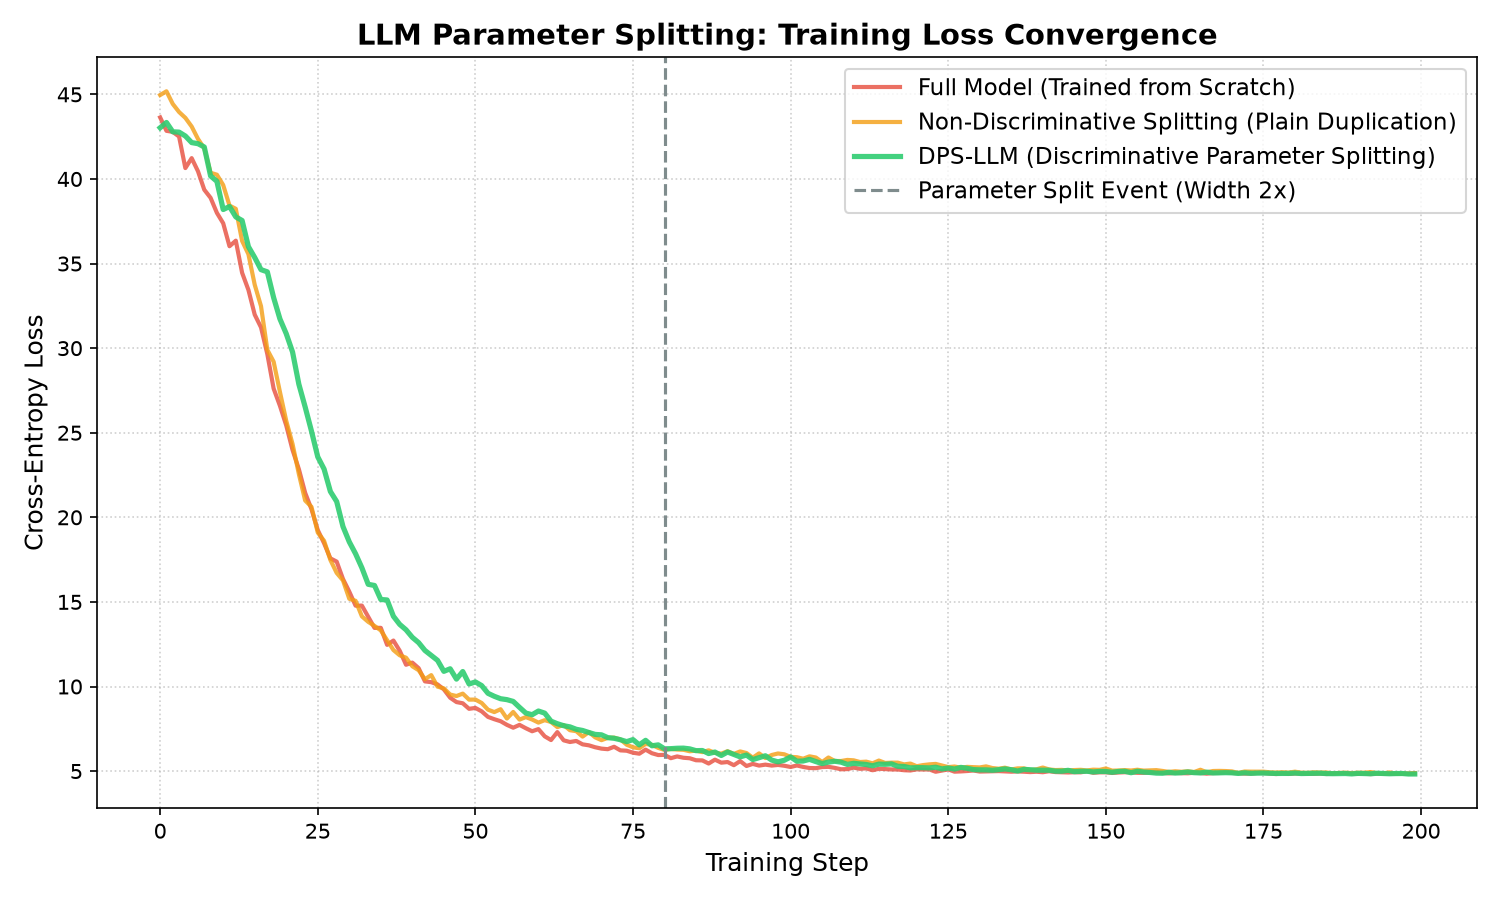
\includegraphics[width=\columnwidth]{dps_llm_training_curve.png}
    \caption{\textbf{Controlled split on a synthetic language-modelling task.} A two-layer SwiGLU Transformer with $d_{ffn}=64$ is trained for 80 steps and then split to $d_{ffn}=128$ (dashed line). Both split variants continue without a loss spike, whereas the $d_{ffn}=128$ model trained from scratch spends its first 80 steps re-learning what the seed already knows. DPS-LLM and plain duplication converge to the same loss as the full model by step 200.}
    \label{fig:training_curve}
\end{figure}

% -----------------------------------------------------------------------------
\section{Related Work}
\paragraph{Function-preserving growth.}
Net2Net \citep{chen2015net2net} introduced \emph{Net2WiderNet} and \emph{Net2DeeperNet}, which widen or deepen a network without changing its function, and noted that a small amount of noise is needed to break the symmetry of copied units. Network morphism \citep{wei2016morphism} generalised the idea to arbitrary non-linear morphisms.
For Transformers, progressive stacking \citep{gong2019stacking} and staged training \citep{shen2022staged} grow depth and width of BERT-style encoders; bert2BERT \citep{chen2022bert2bert} extends Net2Net to attention blocks with function-preserving and advanced knowledge initialisation; LiGO \citep{wang2023ligo} learns a linear growth operator from the small model; MSG \citep{yao2024msg} and LEMON \citep{wang2024lemon} obtain lossless expansion for pre-LayerNorm blocks by masking or by an explicit average-and-cancel construction.
Depth up-scaling \citep{kim2024solar} and HyperCloning \citep{samragh2024hypercloning} apply the same principle to decoder-only LLMs, the latter by tiling weights of a small model into a wider one.
DPS-LLM belongs to this family but targets the gated SwiGLU block specifically, where the $\tfrac{1}{2}$ factor must be placed on the down projection to preserve function.

\paragraph{Neuron splitting.}
Splitting steepest descent \citep{liu2019splitting}, Firefly descent \citep{wu2020firefly} and GradMax \citep{evci2022gradmax} choose \emph{which} neurons to split and \emph{how} to perturb the copies using second-order or gradient information. These methods are principled but require extra computation per split; DPS-LLM instead splits every neuron and uses a closed-form, gradient-free perturbation whose only statistic is the standard deviation of the weight matrix.

\paragraph{Mixture-of-Experts upcycling.}
Sparse upcycling \citep{komatsuzaki2022sparse} initialises MoE experts \citep{shazeer2017outrageously,lepikhin2021gshard,fedus2022switch} by cloning a dense MLP, and \citet{he2024upcycling} study this recipe at scale; Mixtral \citep{jiang2024mixtral} is a widely used dense-to-sparse architecture. Cloned experts are initially identical, so the same symmetry problem arises; our anti-symmetric noise is directly applicable (Appendix~\ref{app:regimes}).

\paragraph{Adapter rank growth.}
LoRA \citep{hu2021lora} fixes the adapter rank in advance; AdaLoRA \citep{zhang2023adalora} and DyLoRA \citep{valipour2023dylora} adapt the rank during training. Rank doubling by parameter splitting (Appendix~\ref{app:regimes}) is a complementary, function-preserving way to increase adapter capacity.

\paragraph{Discriminative splitting in speech.}
\citet{irfan2021discriminative} grew LSTM-RNN acoustic models by duplicating rows and columns of weight matrices and injecting a polarity-preserving perturbation, reporting faster convergence, less over-training and a 1.2\% absolute word-error-rate reduction over Xavier initialisation on a Kaldi/VoxForge recipe. This paper transfers that recipe to Transformers and adds the invariance scaling and the anti-symmetric pairing.

% -----------------------------------------------------------------------------
\section{Method}
\subsection{Function-preserving SwiGLU width splitting}
\label{sec:split}
Modern decoder blocks \citep{shazeer2020glu,touvron2023llama,qwen2024technical} use a gated feed-forward network
\begin{equation}
    \mathrm{FFN}(x) = W_{down}\,\big(\mathrm{SiLU}(W_{gate}x) \odot W_{up}x\big),
    \label{eq:swiglu}
\end{equation}
with $W_{gate},W_{up}\in\mathbb{R}^{d_{ffn}\times d_{model}}$, $W_{down}\in\mathbb{R}^{d_{model}\times d_{ffn}}$, and $\mathrm{SiLU}(z)=z\,\sigma(z)$ \citep{hendrycks2016gelu,elfwing2018silu,ramachandran2017swish}. Let $h(x)=\mathrm{SiLU}(W_{gate}x)\odot W_{up}x\in\mathbb{R}^{d_{ffn}}$.

To grow $d_{ffn}\to 2d_{ffn}$ we apply \emph{rows extension} to the two incoming projections and \emph{columns extension} with a $\tfrac{1}{2}$ factor to the outgoing projection:
\begin{align}
    W_{gate}^{\prime} &= \begin{bmatrix} W_{gate}+\Delta_{gate}^{(1)} \\ W_{gate}+\Delta_{gate}^{(2)} \end{bmatrix}, \label{eq:rows}\\
    W_{up}^{\prime} &= \begin{bmatrix} W_{up}+\Delta_{up}^{(1)} \\ W_{up}+\Delta_{up}^{(2)} \end{bmatrix}, \label{eq:rows_up}\\
    W_{down}^{\prime} &= \tfrac{1}{2}\begin{bmatrix} W_{down} & W_{down} \end{bmatrix} \nonumber\\
    &\quad + \begin{bmatrix} \Delta_{down}^{(1)} & \Delta_{down}^{(2)} \end{bmatrix}. \label{eq:cols}
\end{align}

\begin{theorem}[Functional invariance]
\label{thm:invariance}
With $\Delta=0$, $\mathrm{FFN}'(x)=\mathrm{FFN}(x)$ for every input $x$.
\end{theorem}
\begin{proof}
The stacked gate and up projections produce $[h(x);\,h(x)]$, so
$\mathrm{FFN}'(x)=\tfrac{1}{2}W_{down}h(x)+\tfrac{1}{2}W_{down}h(x)=W_{down}h(x)$.
\end{proof}
Because every block is invariant and the residual stream, attention and normalisation layers are untouched, the whole model is invariant; the loss on any batch is unchanged in exact arithmetic. Without the $\tfrac{1}{2}$ factor the block's output would double, which is the loss spike observed when SwiGLU networks are naively widened.

\subsection{Calculated Anti-Symmetric Noise}
\label{sec:noise}
If $\Delta=0$, the two copies of every neuron are identical and receive identical gradients for the rest of training, so the expanded model has no more effective capacity than the seed \citep{chen2015net2net}.
Isotropic Gaussian noise breaks the tie but is sign-agnostic: it flips the polarity of small weights, which \citet{irfan2021discriminative} found harmful for pre-trained LSTMs.
We instead use a perturbation whose sign is dictated by the weight it perturbs. For a weight matrix $W$ with element-wise standard deviation $\sigma_W$, draw $u\sim\mathcal{U}(0,1)$ and $n\sim\mathcal{N}(0,1)$ independently per element and set
\begin{align}
    f(W) &= \big|(u-\tfrac{1}{2})\cdot C\,\sigma_W\cdot n\big|, \label{eq:f}\\
    \delta(W) &= \mathrm{sign}(W)\odot f(W), \label{eq:delta}\\
    \Delta^{(1)} &= +\delta(W), \qquad \Delta^{(2)} = -\delta(W). \label{eq:pair}
\end{align}
The modulation constant $C=10^{-4}$ is inherited from the original speech recipe; \eqref{eq:f}--\eqref{eq:delta} are its Equations 5.7--5.8 with the noise scaled by $\sigma_W$ so that the same $C$ transfers across layers of different magnitude. Equation~\eqref{eq:pair} is new: the two copies receive \emph{opposite} perturbations. For $W_{down}$ the noise is computed on the already-halved matrix.

\begin{proposition}[Sign preservation]
\label{prop:sign}
Copy 1 satisfies $|w+\delta(w)|=|w|+f(w)>|w|$ for every weight, so no sign is flipped. Copy 2 satisfies $|w-\delta(w)|=\big||w|-f(w)\big|$ and flips sign only if $|w|<f(w)$.
\end{proposition}
Since $f(w)\leq\tfrac{1}{2}C\sigma_W|n|$, a flip requires $|w|<\tfrac{1}{2}\cdot10^{-4}\sigma_W|n|$; for approximately Gaussian weights this is a fraction on the order of $10^{-4}$ of the matrix or less, and these weights carry negligible signal. In our runs the measured sign-flip fraction is $8$--$9\times10^{-6}$ (Section~\ref{sec:results}).

\begin{proposition}[First-order drift cancellation]
\label{prop:drift}
With the pairing in \eqref{eq:pair}, $\mathrm{FFN}'(x)=\mathrm{FFN}(x)+O(\|\delta\|^2)$.
\end{proposition}
\begin{proof}
Write $h_{1}(x)$ and $h_{2}(x)$ for the hidden activations of the two copies. A first-order expansion in $\delta$ gives $h_{1}=h+J\delta x+O(\delta^2)$ and $h_{2}=h-J\delta x+O(\delta^2)$ for the same Jacobian $J$, so $\tfrac{1}{2}W_{down}(h_{1}+h_{2})=W_{down}h+O(\delta^2)$. The down-projection perturbation contributes $\delta_{down}h_{1}-\delta_{down}h_{2}=\delta_{down}(h_{1}-h_{2})=O(\delta^2)$.
\end{proof}
The perturbation therefore does two things at once: it leaves the output unchanged to first order, and it makes $\nabla_{W^{(1)}}\mathcal{L}\neq\nabla_{W^{(2)}}\mathcal{L}$ from the very first update, because the two copies now see different pre-activations. Both statements assume that the perturbation is representable in the weight format. bfloat16 keeps 8 significant bits, so a perturbation of relative size $10^{-4}$ is rounded away for all but the smallest weights; Section~\ref{sec:results} shows that this is what happens in practice.

\subsection{An exact split changes the effective learning rate}
\label{sec:lr_equiv}
Function preservation holds at the moment of the split, but not along the optimisation trajectory. With Adam-type optimisers \citep{kingma2015adam,loshchilov2019adamw}, the split also changes the effective step size of the block.
\begin{proposition}[Split as learning-rate doubling]
\label{prop:lr}
Let the split be exact ($\Delta=0$) and let both models be trained with Adam at learning rate $\eta$. Then, up to Adam's $\epsilon$, the copies stay identical and the split model follows the trajectory of the unsplit model trained with learning rate $\eta$ on $W_{gate},W_{up}$ and $2\eta$ on $W_{down}$.
\end{proposition}
\begin{proof}[Proof sketch]
While the copies are identical, each copy of a row of $W_{gate}$ or $W_{up}$ receives exactly half the gradient of the original row, because it feeds a down-projection column scaled by $\tfrac{1}{2}$; Adam's update is invariant to a constant rescaling of the gradient, so both copies take the step the original would take, and stay identical. Each copy of a column of $W_{down}$ receives the full gradient of the original column, because it sees the same activation; both copies take the original's step, and the effective matrix $W^{(1)}_{down}+W^{(2)}_{down}$ moves twice as far.
\end{proof}
The equivalence is exact in exact arithmetic without gradient clipping and with decoupled weight decay ignored; global-norm clipping, which rescales all gradients jointly, and finite precision make it approximate. On a toy SwiGLU block trained with AdamW in float32 for 100 steps, the losses of the exact split and of the unsplit block with a $2\times$ learning rate on $W_{down}$ differ by at most $7\times10^{-6}$, against $2.4\times10^{-2}$ from the unsplit block at the original learning rate. Comparisons between a split model and its seed at one shared learning rate therefore conflate added capacity with a larger step on $W_{down}$.

\subsection{Applying the operator to a pre-trained LLM}
The split is applied in place to every decoder layer of a Hugging Face checkpoint \citep{wolf2020transformers}: the three linear layers are replaced by their expanded versions and \texttt{intermediate\_size} is doubled in the configuration. No other tensors change. For Qwen2.5-0.5B this grows $d_{ffn}$ from 4864 to 9728 in all 24 layers (+313.8M parameters); for SmolLM-360M from 2560 to 5120 in all 32 layers (+236.0M).

% -----------------------------------------------------------------------------
\begin{table*}[t]
\centering
\small
\setlength{\tabcolsep}{4pt}
\caption{\textbf{Fine-tuning benchmark on two open-weight LLMs and two datasets}, mean $\pm$ standard deviation over three seeds. All runs use the identical budget of Table~\ref{tab:hparams}. \emph{Init PPL} is validation perplexity immediately after splitting and before any update; \emph{Rel.\ PPL reduction} is $100\,(\mathrm{PPL}_{init}-\mathrm{PPL}_{final})/\mathrm{PPL}_{init}$ (higher is better); \emph{Acc.} is GSM8K exact-match accuracy on 100 test problems after fine-tuning. Bold marks the best mean per block.}
\label{tab:empirical_results}
\vspace{2pt}
\begin{tabular*}{\textwidth}{@{\extracolsep{\fill}}llcccccc@{}}
\toprule
\textbf{Model} & \textbf{Dataset} & \textbf{Growth method} & \textbf{Params} & \textbf{Init PPL} & \textbf{Final PPL} & \textbf{Rel.\ PPL red.\ (\%)} & \textbf{Acc.\ (\%)} \\
\midrule
Qwen2.5-0.5B & GSM8K & Base (no split)       & 494.0M & 4.15 & 3.69 $\pm$ 0.05 & 11.18 $\pm$ 1.12 & \textbf{23.0 $\pm$ 2.6} \\
             &       & Naive split ($C{=}0$) & 807.8M & 4.16 & \textbf{3.63 $\pm$ 0.01} & \textbf{12.67 $\pm$ 0.31} & 13.7 $\pm$ 6.7 \\
             &       & Gaussian split        & 807.8M & 4.16 & 3.67 $\pm$ 0.02 & 11.82 $\pm$ 0.41 & 12.7 $\pm$ 4.2 \\
             &       & DPS-LLM (ours)        & 807.8M & 4.16 & 3.66 $\pm$ 0.02 & 11.94 $\pm$ 0.58 & 12.3 $\pm$ 9.0 \\
\midrule
SmolLM-360M  & GSM8K & Base (no split)       & 361.8M & 5.28 & 5.00 $\pm$ 0.01 & 5.25 $\pm$ 0.14 & \textbf{3.7 $\pm$ 1.5} \\
             &       & Naive split ($C{=}0$) & 597.8M & 5.27 & \textbf{4.72 $\pm$ 0.02} & \textbf{10.52 $\pm$ 0.29} & 2.7 $\pm$ 0.6 \\
             &       & Gaussian split        & 597.8M & 5.28 & 4.72 $\pm$ 0.01 & 10.51 $\pm$ 0.29 & 3.3 $\pm$ 1.2 \\
             &       & DPS-LLM (ours)        & 597.8M & 5.27 & 4.72 $\pm$ 0.02 & 10.50 $\pm$ 0.39 & 3.3 $\pm$ 1.2 \\
\midrule
Qwen2.5-0.5B & Alpaca & Base (no split)       & 494.0M & 6.28 & \textbf{4.54 $\pm$ 0.02} & \textbf{27.74 $\pm$ 0.28} & -- \\
             &        & Naive split ($C{=}0$) & 807.8M & 6.27 & 4.67 $\pm$ 0.02 & 25.57 $\pm$ 0.28 & -- \\
             &        & Gaussian split        & 807.8M & 6.27 & 4.66 $\pm$ 0.02 & 25.69 $\pm$ 0.23 & -- \\
             &        & DPS-LLM (ours)        & 807.8M & 6.27 & 4.66 $\pm$ 0.02 & 25.68 $\pm$ 0.34 & -- \\
\midrule
SmolLM-360M  & Alpaca & Base (no split)       & 361.8M & 7.26 & 6.93 $\pm$ 0.00 & 4.57 $\pm$ 0.05 & -- \\
             &        & Naive split ($C{=}0$) & 597.8M & 7.25 & 6.43 $\pm$ 0.01 & 11.39 $\pm$ 0.18 & -- \\
             &        & Gaussian split        & 597.8M & 7.25 & \textbf{6.42 $\pm$ 0.01} & \textbf{11.45 $\pm$ 0.09} & -- \\
             &        & DPS-LLM (ours)        & 597.8M & 7.26 & 6.43 $\pm$ 0.01 & 11.36 $\pm$ 0.16 & -- \\
\bottomrule
\end{tabular*}
\end{table*}

\section{Experiments}
\subsection{Setup}
\label{sec:setup}
\paragraph{Models.}
We use two instruction-tuned open-weight checkpoints that fit on a single 16\,GB GPU after splitting: \texttt{Qwen/Qwen2.5-0.5B-Instruct} \citep{qwen2024technical} (24 layers, $d_{model}=896$, $d_{ffn}=4864$) and \texttt{HuggingFaceTB/SmolLM-360M-Instruct} \citep{allal2024smollm,allal2025smollm2} (32 layers, $d_{model}=960$, $d_{ffn}=2560$). Both use SwiGLU blocks of the form in \eqref{eq:swiglu}.

\paragraph{Datasets.}
GSM8K \citep{cobbe2021gsm8k} (grade-school maths word problems with multi-step solutions) and Alpaca-Cleaned \citep{taori2023alpaca,yahma2023alpacacleaned} (general instruction following), rendered with a fixed template (Appendix~\ref{app:prompts}). For GSM8K we fine-tune on 512 examples drawn from the training split and measure perplexity on the first 200 problems of the test split. For Alpaca-Cleaned, which has no test split, a fixed permutation of the training split provides 512 fine-tuning examples and a disjoint set of 200 validation examples. The data split is fixed (data seed 0) and identical for every condition and run seed.

\paragraph{Growth conditions.}
(1) \emph{Base}: the unmodified checkpoint. (2) \emph{Naive split}: Eqs.~\eqref{eq:rows}--\eqref{eq:cols} with $\Delta=0$, i.e.\ exact duplication with the $\tfrac{1}{2}$ scaling. (3) \emph{Gaussian split}: the same split with i.i.d.\ Gaussian noise drawn independently for each copy, in the spirit of Net2Net \citep{chen2015net2net}, with standard deviation $C\sigma_W/\sqrt{12}$ so that its RMS matches that of the calculated noise. (4) \emph{DPS-LLM}: Calculated Anti-Symmetric Noise with $C=10^{-4}$.

\paragraph{Fine-tuning and evaluation.}
Every condition is fine-tuned with the same recipe (Table~\ref{tab:hparams}). Only the SwiGLU parameters ($W_{gate},W_{up},W_{down}$ of every layer) are updated; attention, embeddings and the output head are frozen so that the comparison isolates the expanded block. Validation perplexity \citep{jelinek1977perplexity} is $\exp$ of the mean per-sequence cross-entropy over the 200 held-out sequences, measured before the first update (\emph{Init PPL}) and after the last (\emph{Final PPL}). GSM8K accuracy is exact match of the final number, generated greedily (at most 256 new tokens) from the prompt ``\texttt{Question: \{question\}\textbackslash nAnswer:}'' for the first 100 test problems. Each run is repeated with seeds 42, 43 and 44, which set the noise draw and the order of the training examples; we report mean $\pm$ standard deviation and a paired $t$-test of DPS-LLM against the naive split across seeds. To quantify symmetry breaking we track, every 25 steps, the mean cosine similarity between the two copies of every split neuron (rows of $W_{gate}$ and $W_{up}$, columns of $W_{down}$).

\begin{table}[t]
\centering
\footnotesize
\setlength{\tabcolsep}{4pt}
\begin{tabular}{@{}lp{0.62\columnwidth}@{}}
\toprule
\textbf{Setting} & \textbf{Value} \\
\midrule
Hardware & Kaggle, 2$\times$ NVIDIA T4 (16\,GB); the two models run concurrently, one per GPU \\
Precision & bfloat16 weights, activations and optimiser state (no fp32 master weights) \\
Optimiser & AdamW \citep{loshchilov2019adamw}, $\beta{=}(0.9,0.999)$, weight decay $0.01$ \\
Learning rate & $2\times10^{-5}$, constant, no warm-up \\
Budget & 200 sequences (batch 1, accumulation 2 $\Rightarrow$ 100 updates), less than one epoch \\
Grad.\ clipping & global norm 1.0 \\
Max seq.\ length & 256 tokens \\
Trainable & SwiGLU MLP of every layer; rest frozen \\
Memory & gradient checkpointing \citep{chen2016checkpointing} \\
Noise constant & $C{=}10^{-4}$ (DPS-LLM, Gaussian); $C{=}0$ (naive) \\
Data & 512 train / 200 validation sequences; 100 GSM8K test problems for accuracy \\
Seeds & 42, 43, 44 (noise draw, example order); data seed 0 \\
Software & PyTorch \citep{paszke2019pytorch}, Transformers \citep{wolf2020transformers}, Datasets \citep{lhoest2021datasets} \\
\bottomrule
\end{tabular}
\caption{Fine-tuning hyper-parameters shared by all 48 benchmark runs.}
\label{tab:hparams}
\end{table}

\begin{figure*}[t]
    \centering
    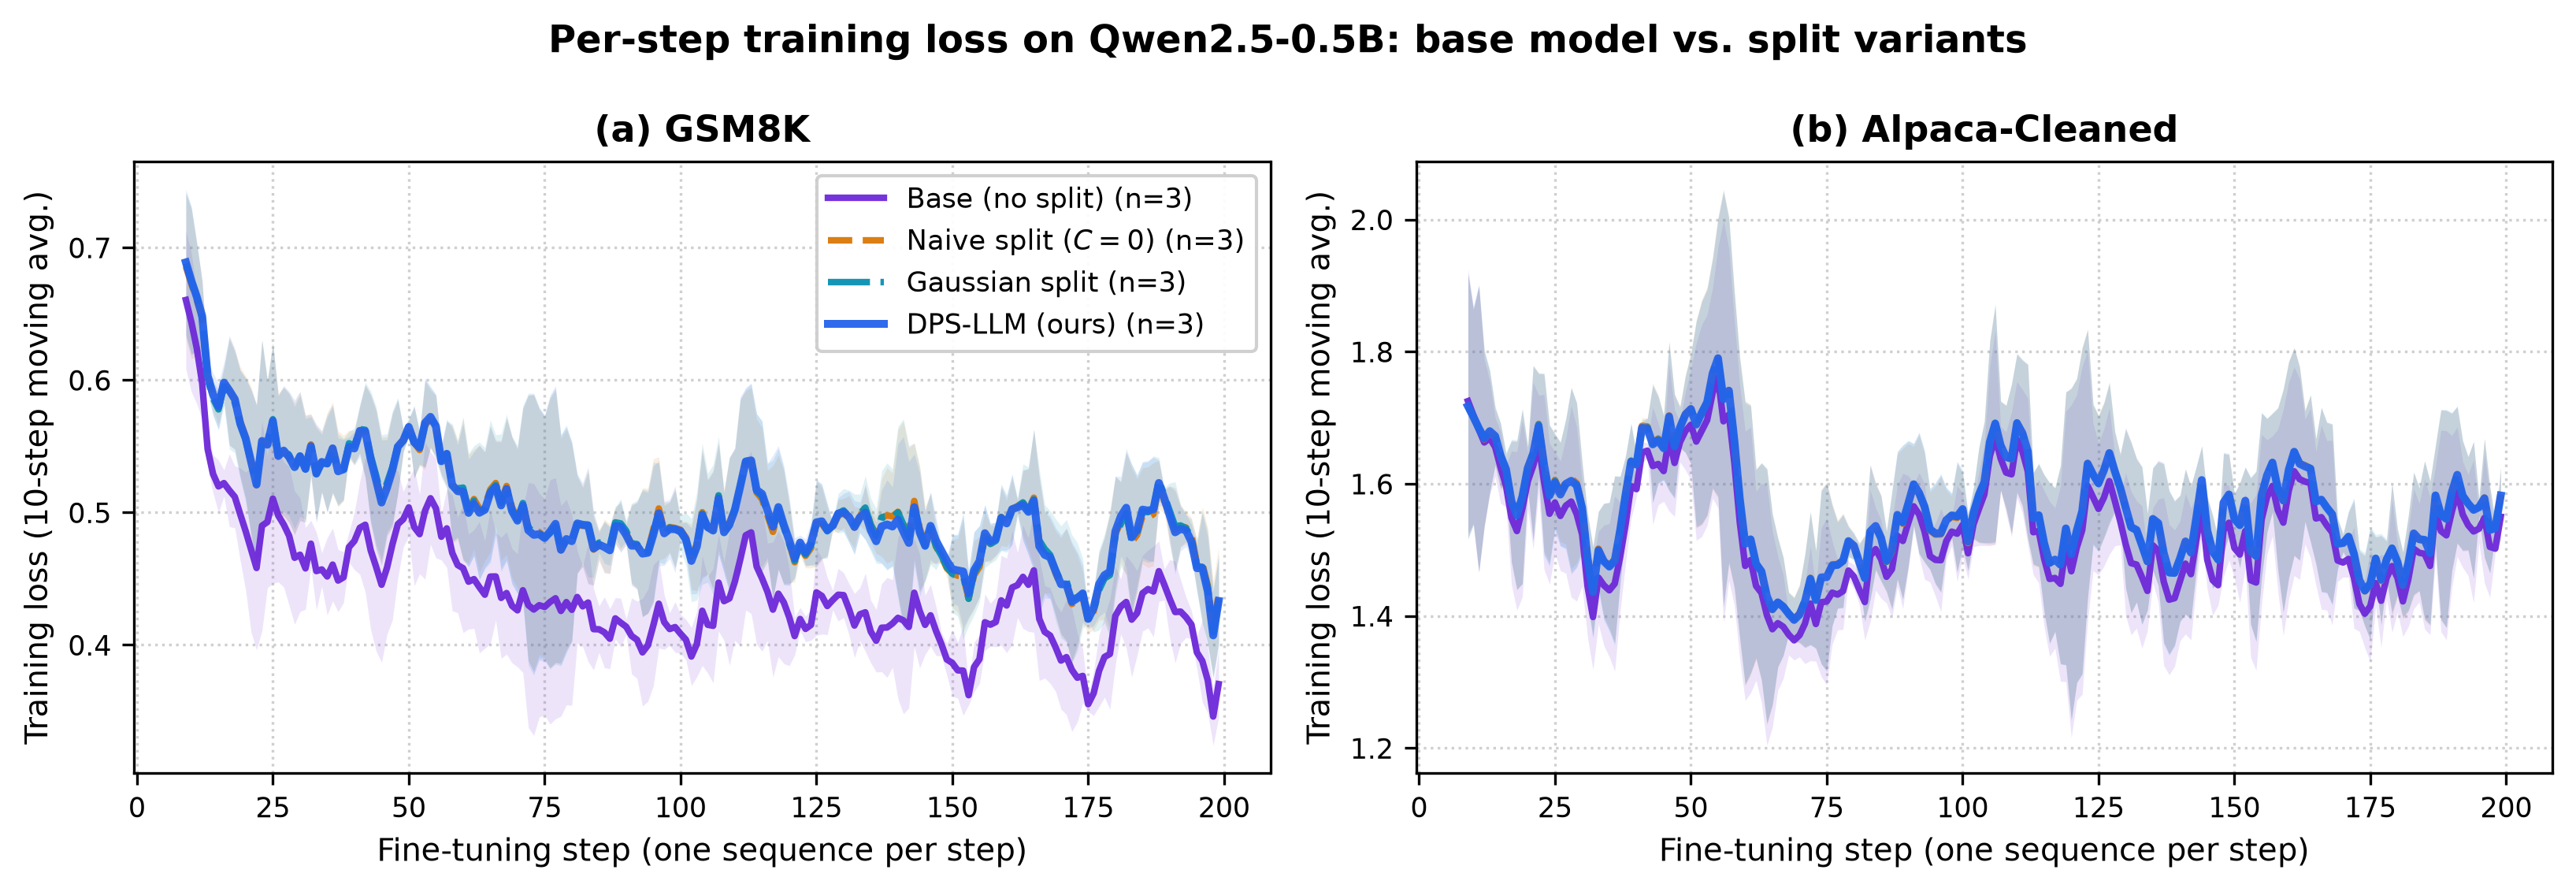
\includegraphics[width=0.72\textwidth]{benchmark_loss_convergence.png}
    \caption{\textbf{Training loss on Qwen2.5-0.5B}, 10-step moving average, mean $\pm$ std over three seeds. All conditions start from the same loss, so the split causes no loss spike. The three split variants are indistinguishable throughout; on GSM8K the unexpanded model reaches a lower training loss than all of them.}
    \label{fig:loss_convergence}
\end{figure*}

\subsection{Results}
\label{sec:results}
Table~\ref{tab:empirical_results} reports the 48 benchmark runs, Figure~\ref{fig:benchmark_results} shows the per-seed comparison with exact duplication, Figure~\ref{fig:loss_convergence} the training loss on Qwen2.5-0.5B, and Table~\ref{tab:ablation} the ablations on SmolLM-360M/GSM8K.

\paragraph{Functional invariance holds on real checkpoints.}
Immediately after splitting, validation perplexity differs from that of the base model by at most $0.012$ in every run, for naive duplication as well as for the noisy splits, so the residual stems from re-associating bfloat16 sums over a hidden dimension twice as wide rather than from the noise. Removing the $\tfrac{1}{2}$ factor on the down projection raises the initial perplexity from $5.27$ to $14.85$ (Table~\ref{tab:ablation}), the loss spike that Theorem~\ref{thm:invariance} avoids.

\paragraph{In bfloat16 the copies never diverge.}
For every split run the mean cosine similarity between the two copies of each neuron is $1.0000$ (to four decimals) at the split and at every checkpoint up to step 200, for DPS-LLM and Gaussian noise as well as for exact duplication. The reason is precision: bfloat16 resolves relative differences of about $2^{-8}\approx0.4\%$, so a perturbation of relative size $10^{-4}$ survives rounding only on the smallest weights. Emulating bfloat16 rounding on $\mathcal{N}(0,0.02^2)$ weights, the copies differ in $0.6\%$ of entries at $C=10^{-4}$ and their cosine similarity is $1.0000$; at $C=10^{-2}$ and $10^{-1}$ the emulation gives $0.99998$ and $0.9988$, which match the values measured after fine-tuning in the ablation (Table~\ref{tab:ablation}). The copies are thus slightly different only when the noise is large enough to be representable, and fine-tuning does not drive them further apart.

\paragraph{DPS-LLM, Gaussian noise and duplication are indistinguishable.}
Consistent with the identical copies, the three split variants reach the same perplexity within seed variation in every setting (Table~\ref{tab:empirical_results}, Figure~\ref{fig:benchmark_results}b). The mean margin of DPS-LLM over the naive split is $-0.73$, $-0.02$, $+0.11$ and $-0.03$ percentage points on Qwen/GSM8K, SmolLM/GSM8K, Qwen/Alpaca and SmolLM/Alpaca; DPS-LLM wins 1, 2, 3 and 1 of the 3 seeds, and no difference is significant (paired $t$-test, $p=0.29$, $0.73$, $0.09$, $0.56$). Differences of this size between conditions whose weights are nearly identical indicate the run-to-run variability of the protocol. The ablation likewise shows no consistent effect of the noise scale ($C$ from $10^{-5}$ to $10^{-1}$), of calculated versus Gaussian noise, or of anti-symmetric versus symmetric pairing.

\paragraph{Splitting changes optimisation, not capacity.}
Splitting doubles the relative perplexity reduction of SmolLM-360M ($5.25\%\to10.5\%$ on GSM8K, $4.57\%\to11.4\%$ on Alpaca), slightly improves Qwen2.5-0.5B on GSM8K ($11.18\%\to11.9$--$12.7\%$) and lowers it on Alpaca ($27.74\%\to25.6$--$25.7\%$). Because the two copies remain identical, a split model represents exactly the same function class as its seed, so none of these differences can be attributed to added capacity. Proposition~\ref{prop:lr} accounts for them: with identical copies, every split variant trains like its seed with a doubled learning rate on $W_{down}$, and the learning-rate ablation shows that this protocol is strongly learning-rate-limited, with the relative perplexity reduction of the split SmolLM rising from $1.85\%$ at $10^{-5}$ to $28.9\%$ at $10^{-4}$ (Table~\ref{tab:ablation}). A larger step helps the slowly adapting SmolLM; on Qwen2.5-0.5B, which adapts much faster at the shared learning rate, it helps slightly on GSM8K and hurts on Alpaca. The equivalence is only approximate here, because gradient clipping is active and bfloat16 rounding differs between the full and the halved down projection, and on Qwen2.5-0.5B/GSM8K the unexpanded model reaches a lower training loss than the split variants (Figure~\ref{fig:loss_convergence}). The decisive control, the unexpanded model trained with a doubled learning rate on $W_{down}$, was not part of this benchmark.

\paragraph{Splitting lowers GSM8K accuracy on Qwen2.5-0.5B.}
After fine-tuning, the unexpanded Qwen2.5-0.5B solves $23.0\%$ of the 100 test problems, while all three split variants solve $12.3$--$13.7\%$, despite reaching similar or lower perplexity on the test solutions. The seed variation is large ($\pm4$--$9$ points), but for every seed the unexpanded model beats every split variant. SmolLM-360M is near the floor ($2.7$--$3.7\%$) in every condition. Lower perplexity on reference solutions therefore does not translate into better problem solving here.

\begin{table}[t]
\centering
\footnotesize
\setlength{\tabcolsep}{3pt}
\begin{tabular}{@{}lcccc@{}}
\toprule
\textbf{Variant} & \textbf{Init} & \textbf{Rel.\ red.} & \textbf{Flips} & \textbf{Pair cos} \\
 & \textbf{PPL} & \textbf{(\%)} & & \textbf{(final)} \\
\midrule
Base (no split)            & 5.28  & 2.92  & --                 & -- \\
Naive split                & 5.27  & 6.24  & 0                  & 1.0000 \\
\midrule
DPS, $C{=}10^{-5}$          & 5.28  & 6.21  & $8.0{\times}10^{-7}$ & 1.0000 \\
DPS, $C{=}10^{-4}$          & 5.27  & 6.24  & $8.3{\times}10^{-6}$ & 1.0000 \\
DPS, $C{=}10^{-3}$          & 5.28  & 6.26  & $8.2{\times}10^{-5}$ & 1.0000 \\
DPS, $C{=}10^{-2}$          & 5.28  & 6.29  & $8.2{\times}10^{-4}$ & 0.99998 \\
DPS, $C{=}10^{-1}$          & 5.28  & 6.19  & $8.2{\times}10^{-3}$ & 0.9988 \\
Gaussian, $C{=}10^{-4}$     & 5.28  & 6.31  & $9.3{\times}10^{-6}$ & 1.0000 \\
Gaussian, $C{=}10^{-2}$     & 5.28  & 6.29  & $9.5{\times}10^{-4}$ & 0.99999 \\
Gaussian, $C{=}10^{-1}$     & 5.29  & 5.97  & $9.5{\times}10^{-3}$ & 0.9991 \\
\midrule
DPS, symmetric $(+\delta,+\delta)$ & 5.28 & 6.26 & 0              & 1.0000 \\
DPS, no $\tfrac{1}{2}$ factor & 14.85 & 10.25 & $8.3{\times}10^{-6}$ & 1.0000 \\
\midrule
DPS, lr $10^{-5}$           & 5.27  & 1.85  & $8.3{\times}10^{-6}$ & -- \\
DPS, lr $5{\times}10^{-5}$  & 5.27  & 18.70 & $8.3{\times}10^{-6}$ & -- \\
DPS, lr $10^{-4}$           & 5.27  & 28.89 & $8.3{\times}10^{-6}$ & -- \\
\bottomrule
\end{tabular}
\caption{\textbf{Ablations} on SmolLM-360M/GSM8K, seed 42, 100 steps (otherwise as Table~\ref{tab:hparams}; default lr $2{\times}10^{-5}$, $C{=}10^{-4}$). \emph{Flips}: fraction of $W_{gate},W_{up}$ entries whose sign the split changes. \emph{Pair cos}: mean cosine similarity of the two copies of each neuron after fine-tuning. Gaussian $C{=}10^{-5}$ and $10^{-3}$ behave like $10^{-4}$ and are omitted.}
\label{tab:ablation}
\end{table}

\begin{figure*}[t]
    \centering
    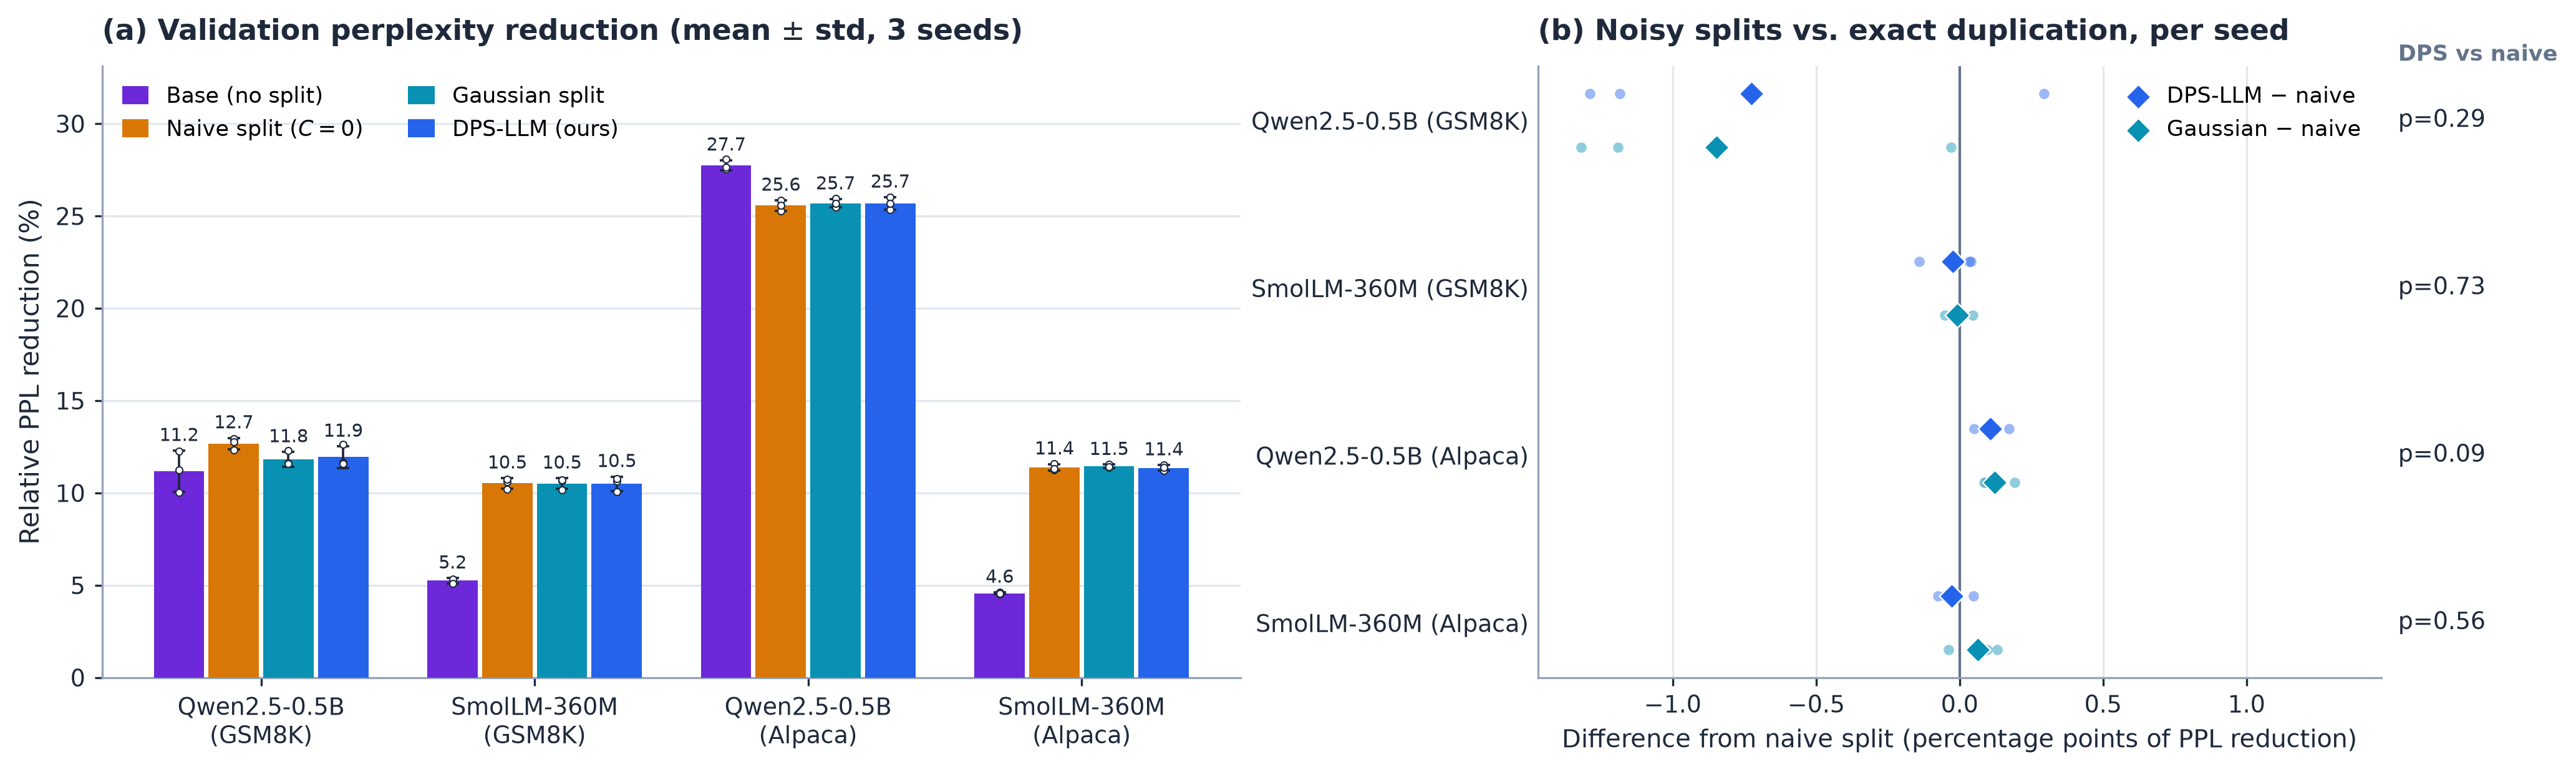
\includegraphics[width=\textwidth]{multi_model_benchmark_comparison.png}
    \caption{\textbf{Benchmark summary.} (a) Relative validation perplexity reduction after fine-tuning, mean $\pm$ std over three seeds, with individual seeds as dots. (b) Per-seed difference of DPS-LLM and Gaussian noise from exact duplication (dots), their mean (diamonds), and the paired $t$-test $p$-value for DPS-LLM. All differences straddle zero.}
    \label{fig:benchmark_results}
\end{figure*}


% -----------------------------------------------------------------------------
\section{Conclusion}
The function-preserving half of DPS-LLM works as intended: placing the invariance factor $\tfrac{1}{2}$ on the down projection grows the SwiGLU blocks of a pre-trained LLM in place, without a loss spike, and removing it raises perplexity almost threefold. The symmetry-breaking half does not take effect in the regime we tested. At $C=10^{-4}$ the calculated noise is below bfloat16 resolution, the two copies of every neuron stay identical through fine-tuning, and DPS-LLM is indistinguishable from exact duplication and from Gaussian noise. The perplexity gains we observe after splitting, up to $2.5\times$ on SmolLM-360M, therefore cannot be credited to added capacity, since under Adam an exact split trains like its seed with a doubled learning rate on $W_{down}$; they also come with a drop in GSM8K accuracy on Qwen2.5-0.5B. A fair evaluation of splitting needs three changes, which our released notebook now implements: the unexpanded model with a doubled learning rate on $W_{down}$ as the matched control; a learning-rate sweep for both the seed and the split model; and weights precise enough for the noise to be representable (float32, or bfloat16 with stochastic rounding and a larger $C$), evaluated on more and larger models. The same operator applies to MoE upcycling and LoRA rank growth, which remain to be evaluated.

% -----------------------------------------------------------------------------
\section*{Limitations}
\textbf{Precision.} All runs fine-tune in pure bfloat16 without fp32 master weights. This makes the default noise ineffective, and many updates smaller than half a bfloat16 unit in the last place are lost in every condition; conclusions about the noise may change once it is representable.
\textbf{Scale of the evidence.} Each condition was fine-tuned on 512 examples for 200 steps (100 optimiser updates) with three seeds; the ablations use one seed and 100 steps. Three seeds detect only large effects, and the paired tests are under-powered for margins below about one percentage point.
\textbf{Learning rate.} The learning rate was fixed across conditions and was swept only for the split model. The benchmark lacks the matched control of Proposition~\ref{prop:lr}, so the comparison with the unexpanded models is confounded by the split's doubled effective learning rate on $W_{down}$.
\textbf{Metrics.} We report perplexity and GSM8K exact match on 100 problems; we do not measure instruction-following quality for Alpaca-Cleaned. GSM8K accuracy was measured only after fine-tuning, not for the checkpoints before it.
\textbf{Data provenance.} The Alpaca-Cleaned validation examples come from its training split; they are unseen during our fine-tuning but may have been seen during the checkpoints' original training.
\textbf{Model scale and regimes.} Both models are below one billion parameters, only width splitting was evaluated, and only the MLP parameters were trained. Depth growth, attention-head splitting, the MoE and LoRA regimes, and full-parameter fine-tuning are untested.
\textbf{Reproducibility.} The two models run concurrently in one process and share PyTorch's global random state, so noise draws depend on the seed but are not bit-reproducible between sessions.

\section*{Ethics Statement}
This work modifies the architecture of publicly released language models and uses two public datasets (GSM8K, MIT licence; Alpaca-Cleaned, CC~BY-NC~4.0) and two public checkpoints (Qwen2.5-0.5B-Instruct and SmolLM-360M-Instruct, both Apache~2.0). Growing a model does not change the biases or safety properties of its seed, and a grown model inherits any limitations of the original checkpoint; practitioners should re-run their safety evaluations after expansion. All experiments ran on a free cloud GPU tier with a small compute footprint (about 3.5 GPU-hours for the main benchmark). No human subjects or personal data were involved.

% -----------------------------------------------------------------------------
\bibliography{references}

% -----------------------------------------------------------------------------
\appendix

\section{Additional Growth Regimes}
\label{app:regimes}
The same rows/columns operator and anti-symmetric noise apply to two further situations. Both are implemented in the released code but were not part of the benchmark in Section~\ref{sec:setup}.

\paragraph{Dense-to-MoE upcycling.}
A dense SwiGLU block is cloned into $E$ experts with independent calculated-noise draws $\Delta^{(e)}$ and combined by a top-$k$ softmax router \citep{shazeer2017outrageously,fedus2022switch}:
\begin{align}
    \mathrm{Expert}_e(x) &= \mathrm{SwiGLU}\big(x;\,W+\Delta^{(e)}\big), \\
    g(x) &= \mathrm{Top}\text{-}k\big(\mathrm{softmax}(W_r x)\big).
\end{align} With $k=E$ and a uniform router the layer is initially function-preserving; the perturbations give each expert a distinct gradient trajectory from the first step, which is the failure mode that sparse upcycling \citep{komatsuzaki2022sparse} must otherwise wait for the router to resolve.

\paragraph{LoRA rank doubling.}
For a LoRA adapter $\Delta W = BA$ with $A\in\mathbb{R}^{r\times d_{in}}$, $B\in\mathbb{R}^{d_{out}\times r}$ \citep{hu2021lora}, the rank is grown $r\to2r$ by
\begin{equation}
    A' = \begin{bmatrix} A \\ A+\Delta_A \end{bmatrix}, \qquad
    B' = \begin{bmatrix} B & \Delta_B \end{bmatrix},
\end{equation}
where $\Delta_B$ is calculated noise on a zero matrix, i.e.\ near zero. Because the new columns of $B$ are (near) zero, $B'A' = BA + \Delta_B(A+\Delta_A)\approx BA$, so the adapted function is preserved while the optimiser gains $r$ additional rank-one directions.

\section{Prompt Templates}
\label{app:prompts}
Each example is rendered as plain text and tokenised with the checkpoint's own tokeniser; no chat template is applied.
\begin{center}\small
\begin{tabular}{@{}l>{\ttfamily}p{0.7\columnwidth}@{}}
\toprule
\textbf{Dataset} & \textrm{\textbf{Template}} \\
\midrule
GSM8K & Question: \{question\}\textbackslash n Answer: \{answer\} \\
Alpaca & Instruction: \{instruction\}\textbackslash n [Input: \{input\}\textbackslash n] Response: \{output\} \\
\bottomrule
\end{tabular}
\end{center}
The bracketed \texttt{Input} line is emitted only when the example has a non-empty input field.

\section{Reproducibility}
\label{app:repro}
The split operator (\texttt{split\_huggingface\_llm.py}), the synthetic experiment behind Figure~\ref{fig:training_curve}, and the Kaggle notebook that produced Tables~\ref{tab:empirical_results} and~\ref{tab:ablation} are available at \url{https://github.com/mirfan899/parameter-splitting-llm}, together with every per-seed result, loss history and neuron-pair similarity trace (\texttt{results/full\_2026-10-06}). The 48-run benchmark takes about 3.5 GPU-hours, under two hours of wall-clock time on a free Kaggle session with two T4 GPUs, plus the ablations.

\end{document}
